\documentclass[twoside]{book}

% Packages required by doxygen
\usepackage{fixltx2e}
\usepackage{calc}
\usepackage{doxygen}
\usepackage[export]{adjustbox} % also loads graphicx
\usepackage{graphicx}
\usepackage[utf8]{inputenc}
\usepackage{makeidx}
\usepackage{multicol}
\usepackage{multirow}
\PassOptionsToPackage{warn}{textcomp}
\usepackage{textcomp}
\usepackage[nointegrals]{wasysym}
\usepackage[table]{xcolor}

% Font selection
\usepackage[T1]{fontenc}
\usepackage[scaled=.90]{helvet}
\usepackage{courier}
\usepackage{amssymb}
\usepackage{sectsty}
\renewcommand{\familydefault}{\sfdefault}
\allsectionsfont{%
  \fontseries{bc}\selectfont%
  \color{darkgray}%
}
\renewcommand{\DoxyLabelFont}{%
  \fontseries{bc}\selectfont%
  \color{darkgray}%
}
\newcommand{\+}{\discretionary{\mbox{\scriptsize$\hookleftarrow$}}{}{}}

% Page & text layout
\usepackage{geometry}
\geometry{%
  a4paper,%
  top=2.5cm,%
  bottom=2.5cm,%
  left=2.5cm,%
  right=2.5cm%
}
\tolerance=750
\hfuzz=15pt
\hbadness=750
\setlength{\emergencystretch}{15pt}
\setlength{\parindent}{0cm}
\setlength{\parskip}{0.2cm}
\makeatletter
\renewcommand{\paragraph}{%
  \@startsection{paragraph}{4}{0ex}{-1.0ex}{1.0ex}{%
    \normalfont\normalsize\bfseries\SS@parafont%
  }%
}
\renewcommand{\subparagraph}{%
  \@startsection{subparagraph}{5}{0ex}{-1.0ex}{1.0ex}{%
    \normalfont\normalsize\bfseries\SS@subparafont%
  }%
}
\makeatother

% Headers & footers
\usepackage{fancyhdr}
\pagestyle{fancyplain}
\fancyhead[LE]{\fancyplain{}{\bfseries\thepage}}
\fancyhead[CE]{\fancyplain{}{}}
\fancyhead[RE]{\fancyplain{}{\bfseries\leftmark}}
\fancyhead[LO]{\fancyplain{}{\bfseries\rightmark}}
\fancyhead[CO]{\fancyplain{}{}}
\fancyhead[RO]{\fancyplain{}{\bfseries\thepage}}
\fancyfoot[LE]{\fancyplain{}{}}
\fancyfoot[CE]{\fancyplain{}{}}
\fancyfoot[RE]{\fancyplain{}{\bfseries\scriptsize Generated on Sat Jan 10 2015 04\+:37\+:10 for librcfclient by Doxygen }}
\fancyfoot[LO]{\fancyplain{}{\bfseries\scriptsize Generated on Sat Jan 10 2015 04\+:37\+:10 for librcfclient by Doxygen }}
\fancyfoot[CO]{\fancyplain{}{}}
\fancyfoot[RO]{\fancyplain{}{}}
\renewcommand{\footrulewidth}{0.4pt}
\renewcommand{\chaptermark}[1]{%
  \markboth{#1}{}%
}
\renewcommand{\sectionmark}[1]{%
  \markright{\thesection\ #1}%
}

% Indices & bibliography
\usepackage{natbib}
\usepackage[titles]{tocloft}
\setcounter{tocdepth}{3}
\setcounter{secnumdepth}{5}
\makeindex

% Hyperlinks (required, but should be loaded last)
\usepackage{ifpdf}
\ifpdf
  \usepackage[pdftex,pagebackref=true]{hyperref}
\else
  \usepackage[ps2pdf,pagebackref=true]{hyperref}
\fi
\hypersetup{%
  colorlinks=true,%
  linkcolor=blue,%
  citecolor=blue,%
  unicode%
}

% Custom commands
\newcommand{\clearemptydoublepage}{%
  \newpage{\pagestyle{empty}\cleardoublepage}%
}


%===== C O N T E N T S =====

\begin{document}

% Titlepage & ToC
\hypersetup{pageanchor=false,
             bookmarks=true,
             bookmarksnumbered=true,
             pdfencoding=unicode
            }
\pagenumbering{roman}
\begin{titlepage}
\vspace*{7cm}
\begin{center}%
{\Large librcfclient \\[1ex]\large 0.\+1 }\\
\vspace*{1cm}
{\large Generated by Doxygen 1.8.9.1}\\
\vspace*{0.5cm}
{\small Sat Jan 10 2015 04:37:10}\\
\end{center}
\end{titlepage}
\clearemptydoublepage
\tableofcontents
\clearemptydoublepage
\pagenumbering{arabic}
\hypersetup{pageanchor=true}

%--- Begin generated contents ---
\chapter{Namespace Index}
\section{Namespace List}
Here is a list of all documented namespaces with brief descriptions\+:\begin{DoxyCompactList}
\item\contentsline{section}{\hyperlink{namespace_r_c_f}{R\+C\+F} \\*A global namespace for Remote\+Control\+Framework }{\pageref{namespace_r_c_f}}{}
\item\contentsline{section}{\hyperlink{namespace_r_c_f_1_1_common}{R\+C\+F\+::\+Common} \\*A namespace for common Remote\+Control\+Framework classes }{\pageref{namespace_r_c_f_1_1_common}}{}
\end{DoxyCompactList}

\chapter{Class Index}
\section{Class List}
Here are the classes, structs, unions and interfaces with brief descriptions\+:\begin{DoxyCompactList}
\item\contentsline{section}{\hyperlink{class_r_c_f_1_1_client_1_1_client}{R\+C\+F\+::\+Client\+::\+Client} \\*A class that can be used to create \hyperlink{namespace_r_c_f}{R\+C\+F} client and contains useful \hyperlink{namespace_r_c_f}{R\+C\+F} protocol methods }{\pageref{class_r_c_f_1_1_client_1_1_client}}{}
\item\contentsline{section}{\hyperlink{class_r_c_f_1_1_client_1_1_server_definition}{R\+C\+F\+::\+Client\+::\+Server\+Definition} \\*A class that represents server definition for client }{\pageref{class_r_c_f_1_1_client_1_1_server_definition}}{}
\end{DoxyCompactList}

\chapter{File Index}
\section{File List}
Here is a list of all documented files with brief descriptions\+:\begin{DoxyCompactList}
\item\contentsline{section}{include/\hyperlink{_client_8h}{Client.\+h} \\*A class that can be used to create \hyperlink{namespace_r_c_f}{R\+C\+F} client and contains useful \hyperlink{namespace_r_c_f}{R\+C\+F} protocol methods }{\pageref{_client_8h}}{}
\item\contentsline{section}{include/{\bfseries librcfclient.\+h} }{\pageref{librcfclient_8h}}{}
\item\contentsline{section}{include/\hyperlink{_server_definition_8h}{Server\+Definition.\+h} \\*A class that represents server definition for client }{\pageref{_server_definition_8h}}{}
\end{DoxyCompactList}

\chapter{Namespace Documentation}
\hypertarget{namespace_r_c_f}{}\section{R\+C\+F Namespace Reference}
\label{namespace_r_c_f}\index{R\+C\+F@{R\+C\+F}}


A global namespace for Remote\+Control\+Framework.  


\subsection*{Namespaces}
\begin{DoxyCompactItemize}
\item 
 \hyperlink{namespace_r_c_f_1_1_common}{Common}
\begin{DoxyCompactList}\small\item\em A namespace for common Remote\+Control\+Framework classes. \end{DoxyCompactList}\end{DoxyCompactItemize}


\subsection{Detailed Description}
A global namespace for Remote\+Control\+Framework. 
\hypertarget{namespace_r_c_f_1_1_client}{}\section{R\+C\+F\+:\+:Client Namespace Reference}
\label{namespace_r_c_f_1_1_client}\index{R\+C\+F\+::\+Client@{R\+C\+F\+::\+Client}}


A namespace for \hyperlink{namespace_r_c_f}{R\+C\+F} client.  


\subsection*{Classes}
\begin{DoxyCompactItemize}
\item 
class \hyperlink{class_r_c_f_1_1_client_1_1_client}{Client}
\begin{DoxyCompactList}\small\item\em A class that can be used to create \hyperlink{namespace_r_c_f}{R\+C\+F} client and contains useful \hyperlink{namespace_r_c_f}{R\+C\+F} protocol methods. \end{DoxyCompactList}\item 
class \hyperlink{class_r_c_f_1_1_client_1_1_server_definition}{Server\+Definition}
\begin{DoxyCompactList}\small\item\em A class that represents server definition for client. \end{DoxyCompactList}\end{DoxyCompactItemize}


\subsection{Detailed Description}
A namespace for \hyperlink{namespace_r_c_f}{R\+C\+F} client. 
\chapter{Class Documentation}
\hypertarget{class_r_c_f_1_1_client_1_1_client}{}\section{R\+C\+F\+:\+:Client\+:\+:Client Class Reference}
\label{class_r_c_f_1_1_client_1_1_client}\index{R\+C\+F\+::\+Client\+::\+Client@{R\+C\+F\+::\+Client\+::\+Client}}


A class that can be used to create \hyperlink{namespace_r_c_f}{R\+C\+F} client and contains useful \hyperlink{namespace_r_c_f}{R\+C\+F} protocol methods.  




{\ttfamily \#include $<$Client.\+h$>$}

\subsection*{Public Member Functions}
\begin{DoxyCompactItemize}
\item 
\hyperlink{class_r_c_f_1_1_client_1_1_client_af33c081e68edc60672a985a47a49cbd9}{Client} (boost\+::asio\+::io\+\_\+service \&service, std\+::string sd\+Name)
\begin{DoxyCompactList}\small\item\em A constructor from boost\+::asio\+::io\+\_\+service and server definition name. \end{DoxyCompactList}\item 
\hypertarget{class_r_c_f_1_1_client_1_1_client_a73f3268d395a074869a25507fe19f38e}{}\hyperlink{class_r_c_f_1_1_client_1_1_client_a73f3268d395a074869a25507fe19f38e}{$\sim$\+Client} ()\label{class_r_c_f_1_1_client_1_1_client_a73f3268d395a074869a25507fe19f38e}

\begin{DoxyCompactList}\small\item\em A destructor. \end{DoxyCompactList}\item 
\hyperlink{class_r_c_f_1_1_client_1_1_server_definition}{Server\+Definition} $\ast$ \hyperlink{class_r_c_f_1_1_client_1_1_client_a1459e5b65c1ebdada7a46a8604464099}{get\+Server\+Definition} ()
\begin{DoxyCompactList}\small\item\em Returns the server definition this client has been connected to. \end{DoxyCompactList}\item 
\hypertarget{class_r_c_f_1_1_client_1_1_client_a0948bd7c88f562718ef70cd32360adf5}{}void \hyperlink{class_r_c_f_1_1_client_1_1_client_a0948bd7c88f562718ef70cd32360adf5}{handshake} ()\label{class_r_c_f_1_1_client_1_1_client_a0948bd7c88f562718ef70cd32360adf5}

\begin{DoxyCompactList}\small\item\em Performs the handshake with the server. \end{DoxyCompactList}\item 
void \hyperlink{class_r_c_f_1_1_client_1_1_client_ab08c9ae64d744de85a624a4161e1f8a2}{authorize} (std\+::string username, std\+::string password)
\begin{DoxyCompactList}\small\item\em Authorize the user on the server. \end{DoxyCompactList}\item 
std\+::string \hyperlink{class_r_c_f_1_1_client_1_1_client_ac2995dbb6dd0087d5eb8c874e74c3c6c}{list} ()
\begin{DoxyCompactList}\small\item\em Obtains a list of commands for currently logged in user. \end{DoxyCompactList}\item 
int \hyperlink{class_r_c_f_1_1_client_1_1_client_a47b9ab652ebbe6de0a104f797ce43a92}{execute} (std\+::string query, std\+::string $\ast$stdout\+\_\+target, std\+::string $\ast$stderr\+\_\+target, std\+::string($\ast$param\+Provider)())
\begin{DoxyCompactList}\small\item\em Executes a command on the server. \end{DoxyCompactList}\item 
int \hyperlink{class_r_c_f_1_1_client_1_1_client_a0e2e53ce56c010fb9552c8fa826d2efe}{execute} (std\+::string query, std\+::string $\ast$stdout\+\_\+target, std\+::string $\ast$stderr\+\_\+target, std\+::string($\ast$param\+Provider)(\hyperlink{class_r_c_f_1_1_client_1_1_client}{Client} $\ast$))
\begin{DoxyCompactList}\small\item\em Executes a command on the server. \end{DoxyCompactList}\item 
\hypertarget{class_r_c_f_1_1_client_1_1_client_a07c43c20e56147d36048c33849f8a343}{}void \hyperlink{class_r_c_f_1_1_client_1_1_client_a07c43c20e56147d36048c33849f8a343}{close} ()\label{class_r_c_f_1_1_client_1_1_client_a07c43c20e56147d36048c33849f8a343}

\begin{DoxyCompactList}\small\item\em Closes the connection. \end{DoxyCompactList}\item 
std\+::string \hyperlink{class_r_c_f_1_1_client_1_1_client_addc515db3d84fe809d4b61edca5d08dd}{read} ()
\begin{DoxyCompactList}\small\item\em Reads next portion of the transmission. \end{DoxyCompactList}\item 
void \hyperlink{class_r_c_f_1_1_client_1_1_client_a4a291f266e0336a4a0bad5e87683b583}{write} (std\+::string trans)
\begin{DoxyCompactList}\small\item\em Writes next portion of the transmission, adding the ending separator. \end{DoxyCompactList}\item 
std\+::string \hyperlink{class_r_c_f_1_1_client_1_1_client_a10f181c9a9dd7624b9ae86a88c90f882}{get\+Logged\+Username} ()
\begin{DoxyCompactList}\small\item\em Returns the username used to login. \end{DoxyCompactList}\end{DoxyCompactItemize}


\subsection{Detailed Description}
A class that can be used to create \hyperlink{namespace_r_c_f}{R\+C\+F} client and contains useful \hyperlink{namespace_r_c_f}{R\+C\+F} protocol methods. 

\subsection{Constructor \& Destructor Documentation}
\hypertarget{class_r_c_f_1_1_client_1_1_client_af33c081e68edc60672a985a47a49cbd9}{}\index{R\+C\+F\+::\+Client\+::\+Client@{R\+C\+F\+::\+Client\+::\+Client}!Client@{Client}}
\index{Client@{Client}!R\+C\+F\+::\+Client\+::\+Client@{R\+C\+F\+::\+Client\+::\+Client}}
\subsubsection[{Client}]{\setlength{\rightskip}{0pt plus 5cm}R\+C\+F\+::\+Client\+::\+Client\+::\+Client (
\begin{DoxyParamCaption}
\item[{boost\+::asio\+::io\+\_\+service \&}]{service, }
\item[{std\+::string}]{sd\+Name}
\end{DoxyParamCaption}
)}\label{class_r_c_f_1_1_client_1_1_client_af33c081e68edc60672a985a47a49cbd9}


A constructor from boost\+::asio\+::io\+\_\+service and server definition name. 


\begin{DoxyParams}{Parameters}
{\em service} & A reference to boost\+::asio\+::io\+\_\+service, that has to be constructed before server construction and is used for boost\+::asio communication (refer to boost\+::asio documentation for more information). \\
\hline
{\em sd\+Name} & Server definition name. \\
\hline
\end{DoxyParams}


\subsection{Member Function Documentation}
\hypertarget{class_r_c_f_1_1_client_1_1_client_ab08c9ae64d744de85a624a4161e1f8a2}{}\index{R\+C\+F\+::\+Client\+::\+Client@{R\+C\+F\+::\+Client\+::\+Client}!authorize@{authorize}}
\index{authorize@{authorize}!R\+C\+F\+::\+Client\+::\+Client@{R\+C\+F\+::\+Client\+::\+Client}}
\subsubsection[{authorize}]{\setlength{\rightskip}{0pt plus 5cm}void R\+C\+F\+::\+Client\+::\+Client\+::authorize (
\begin{DoxyParamCaption}
\item[{std\+::string}]{username, }
\item[{std\+::string}]{password}
\end{DoxyParamCaption}
)}\label{class_r_c_f_1_1_client_1_1_client_ab08c9ae64d744de85a624a4161e1f8a2}


Authorize the user on the server. 


\begin{DoxyParams}{Parameters}
{\em username} & A username to authorize with. \\
\hline
{\em password} & A password to authorize with. \\
\hline
\end{DoxyParams}
\hypertarget{class_r_c_f_1_1_client_1_1_client_a47b9ab652ebbe6de0a104f797ce43a92}{}\index{R\+C\+F\+::\+Client\+::\+Client@{R\+C\+F\+::\+Client\+::\+Client}!execute@{execute}}
\index{execute@{execute}!R\+C\+F\+::\+Client\+::\+Client@{R\+C\+F\+::\+Client\+::\+Client}}
\subsubsection[{execute}]{\setlength{\rightskip}{0pt plus 5cm}int R\+C\+F\+::\+Client\+::\+Client\+::execute (
\begin{DoxyParamCaption}
\item[{std\+::string}]{query, }
\item[{std\+::string $\ast$}]{stdout\+\_\+target, }
\item[{std\+::string $\ast$}]{stderr\+\_\+target, }
\item[{std\+::string($\ast$)()}]{param\+Provider}
\end{DoxyParamCaption}
)}\label{class_r_c_f_1_1_client_1_1_client_a47b9ab652ebbe6de0a104f797ce43a92}


Executes a command on the server. 


\begin{DoxyParams}{Parameters}
{\em query} & A command query -\/ includes command name preceded by the hierarchy of groups that command belongs to, separated by \+: sign. Example\+: administration\+:network\+:mycommand, where mycommand belongs to the network group, and network group belongs to administration group which is top-\/level on the server. \\
\hline
{\em stdout\+\_\+target} & A target string where command stdout should be placed. \\
\hline
{\em stderr\+\_\+target} & A target string where command stderr should be placed. \\
\hline
{\em param\+Provider} & A function that provides additional parameters for the command (in response to P\+A\+R\+A\+M protocol message). Takes no arguments, returns std\+::string. \\
\hline
\end{DoxyParams}
\begin{DoxyReturn}{Returns}
Command exit code. 
\end{DoxyReturn}
\hypertarget{class_r_c_f_1_1_client_1_1_client_a0e2e53ce56c010fb9552c8fa826d2efe}{}\index{R\+C\+F\+::\+Client\+::\+Client@{R\+C\+F\+::\+Client\+::\+Client}!execute@{execute}}
\index{execute@{execute}!R\+C\+F\+::\+Client\+::\+Client@{R\+C\+F\+::\+Client\+::\+Client}}
\subsubsection[{execute}]{\setlength{\rightskip}{0pt plus 5cm}int R\+C\+F\+::\+Client\+::\+Client\+::execute (
\begin{DoxyParamCaption}
\item[{std\+::string}]{query, }
\item[{std\+::string $\ast$}]{stdout\+\_\+target, }
\item[{std\+::string $\ast$}]{stderr\+\_\+target, }
\item[{std\+::string($\ast$)({\bf Client} $\ast$)}]{param\+Provider}
\end{DoxyParamCaption}
)}\label{class_r_c_f_1_1_client_1_1_client_a0e2e53ce56c010fb9552c8fa826d2efe}


Executes a command on the server. 


\begin{DoxyParams}{Parameters}
{\em query} & A command query -\/ includes command name preceded by the hierarchy of groups that command belongs to, separated by \+: sign. Example\+: administration\+:network\+:mycommand, where mycommand belongs to the network group, and network group belongs to administration group which is top-\/level on the server. \\
\hline
{\em stdout\+\_\+target} & A target string where command stdout should be placed. \\
\hline
{\em stderr\+\_\+target} & A target string where command stderr should be placed. \\
\hline
{\em param\+Provider} & A function that provides additional parameters for the command (in response to P\+A\+R\+A\+M protocol message). Takes a \hyperlink{class_r_c_f_1_1_client_1_1_client}{Client} argument, returns std\+::string. Can be used if additional information from the client module is needed in the function. \\
\hline
\end{DoxyParams}
\begin{DoxyReturn}{Returns}
Command exit code. 
\end{DoxyReturn}
\hypertarget{class_r_c_f_1_1_client_1_1_client_a10f181c9a9dd7624b9ae86a88c90f882}{}\index{R\+C\+F\+::\+Client\+::\+Client@{R\+C\+F\+::\+Client\+::\+Client}!get\+Logged\+Username@{get\+Logged\+Username}}
\index{get\+Logged\+Username@{get\+Logged\+Username}!R\+C\+F\+::\+Client\+::\+Client@{R\+C\+F\+::\+Client\+::\+Client}}
\subsubsection[{get\+Logged\+Username}]{\setlength{\rightskip}{0pt plus 5cm}std\+::string R\+C\+F\+::\+Client\+::\+Client\+::get\+Logged\+Username (
\begin{DoxyParamCaption}
{}
\end{DoxyParamCaption}
)}\label{class_r_c_f_1_1_client_1_1_client_a10f181c9a9dd7624b9ae86a88c90f882}


Returns the username used to login. 

\begin{DoxyReturn}{Returns}
Logged in username. 
\end{DoxyReturn}
\hypertarget{class_r_c_f_1_1_client_1_1_client_a1459e5b65c1ebdada7a46a8604464099}{}\index{R\+C\+F\+::\+Client\+::\+Client@{R\+C\+F\+::\+Client\+::\+Client}!get\+Server\+Definition@{get\+Server\+Definition}}
\index{get\+Server\+Definition@{get\+Server\+Definition}!R\+C\+F\+::\+Client\+::\+Client@{R\+C\+F\+::\+Client\+::\+Client}}
\subsubsection[{get\+Server\+Definition}]{\setlength{\rightskip}{0pt plus 5cm}{\bf Server\+Definition}$\ast$ R\+C\+F\+::\+Client\+::\+Client\+::get\+Server\+Definition (
\begin{DoxyParamCaption}
{}
\end{DoxyParamCaption}
)}\label{class_r_c_f_1_1_client_1_1_client_a1459e5b65c1ebdada7a46a8604464099}


Returns the server definition this client has been connected to. 

\begin{DoxyReturn}{Returns}
A pointer to \hyperlink{class_r_c_f_1_1_client_1_1_server_definition}{Server\+Definition} which was used to connect. 
\end{DoxyReturn}
\hypertarget{class_r_c_f_1_1_client_1_1_client_ac2995dbb6dd0087d5eb8c874e74c3c6c}{}\index{R\+C\+F\+::\+Client\+::\+Client@{R\+C\+F\+::\+Client\+::\+Client}!list@{list}}
\index{list@{list}!R\+C\+F\+::\+Client\+::\+Client@{R\+C\+F\+::\+Client\+::\+Client}}
\subsubsection[{list}]{\setlength{\rightskip}{0pt plus 5cm}std\+::string R\+C\+F\+::\+Client\+::\+Client\+::list (
\begin{DoxyParamCaption}
{}
\end{DoxyParamCaption}
)}\label{class_r_c_f_1_1_client_1_1_client_ac2995dbb6dd0087d5eb8c874e74c3c6c}


Obtains a list of commands for currently logged in user. 

\begin{DoxyReturn}{Returns}
List of commands to be parsed by the client. 
\end{DoxyReturn}
\hypertarget{class_r_c_f_1_1_client_1_1_client_addc515db3d84fe809d4b61edca5d08dd}{}\index{R\+C\+F\+::\+Client\+::\+Client@{R\+C\+F\+::\+Client\+::\+Client}!read@{read}}
\index{read@{read}!R\+C\+F\+::\+Client\+::\+Client@{R\+C\+F\+::\+Client\+::\+Client}}
\subsubsection[{read}]{\setlength{\rightskip}{0pt plus 5cm}std\+::string R\+C\+F\+::\+Client\+::\+Client\+::read (
\begin{DoxyParamCaption}
{}
\end{DoxyParamCaption}
)}\label{class_r_c_f_1_1_client_1_1_client_addc515db3d84fe809d4b61edca5d08dd}


Reads next portion of the transmission. 

\begin{DoxyReturn}{Returns}
Received data without ending separator as std\+::string. 
\end{DoxyReturn}
\hypertarget{class_r_c_f_1_1_client_1_1_client_a4a291f266e0336a4a0bad5e87683b583}{}\index{R\+C\+F\+::\+Client\+::\+Client@{R\+C\+F\+::\+Client\+::\+Client}!write@{write}}
\index{write@{write}!R\+C\+F\+::\+Client\+::\+Client@{R\+C\+F\+::\+Client\+::\+Client}}
\subsubsection[{write}]{\setlength{\rightskip}{0pt plus 5cm}void R\+C\+F\+::\+Client\+::\+Client\+::write (
\begin{DoxyParamCaption}
\item[{std\+::string}]{trans}
\end{DoxyParamCaption}
)}\label{class_r_c_f_1_1_client_1_1_client_a4a291f266e0336a4a0bad5e87683b583}


Writes next portion of the transmission, adding the ending separator. 


\begin{DoxyParams}{Parameters}
{\em trans} & Transmission to write. \\
\hline
\end{DoxyParams}


The documentation for this class was generated from the following file\+:\begin{DoxyCompactItemize}
\item 
include/\hyperlink{_client_8h}{Client.\+h}\end{DoxyCompactItemize}

\hypertarget{class_r_c_f_1_1_client_1_1_server_definition}{}\section{R\+C\+F\+:\+:Client\+:\+:Server\+Definition Class Reference}
\label{class_r_c_f_1_1_client_1_1_server_definition}\index{R\+C\+F\+::\+Client\+::\+Server\+Definition@{R\+C\+F\+::\+Client\+::\+Server\+Definition}}


A class that represents server definition for client.  




{\ttfamily \#include $<$Server\+Definition.\+h$>$}

\subsection*{Public Member Functions}
\begin{DoxyCompactItemize}
\item 
\hypertarget{class_r_c_f_1_1_client_1_1_server_definition_aac5283639c40891522960d6223bdc10d}{}\hyperlink{class_r_c_f_1_1_client_1_1_server_definition_aac5283639c40891522960d6223bdc10d}{Server\+Definition} ()\label{class_r_c_f_1_1_client_1_1_server_definition_aac5283639c40891522960d6223bdc10d}

\begin{DoxyCompactList}\small\item\em A plain constructor. \end{DoxyCompactList}\item 
\hyperlink{class_r_c_f_1_1_client_1_1_server_definition_a8492b1915c3014b9111fd884160a3bf1}{Server\+Definition} (std\+::string name, std\+::string hostname, std\+::string certfilepath)
\begin{DoxyCompactList}\small\item\em A constructor from name, hostname and certificate file path. \end{DoxyCompactList}\item 
std\+::string \hyperlink{class_r_c_f_1_1_client_1_1_server_definition_a20f355baa25a4945373051b6d6c70efd}{get\+Name} ()
\begin{DoxyCompactList}\small\item\em Returns server definition name. \end{DoxyCompactList}\item 
std\+::string \hyperlink{class_r_c_f_1_1_client_1_1_server_definition_aa7ad5f20250bf2fa557920ef1991e76f}{get\+Hostname} ()
\begin{DoxyCompactList}\small\item\em Returns server hostname. \end{DoxyCompactList}\item 
boost\+::filesystem\+::path \hyperlink{class_r_c_f_1_1_client_1_1_server_definition_a3cb06170956a9bd97523bf54cdee6ab6}{get\+Cert\+File} ()
\begin{DoxyCompactList}\small\item\em Returns a path to server\textquotesingle{} s certificate file. \end{DoxyCompactList}\item 
bool \hyperlink{class_r_c_f_1_1_client_1_1_server_definition_afb97f6e4203ea56890a9b4bdc99ea45c}{valid} ()
\begin{DoxyCompactList}\small\item\em Checks if definition is valid to save or process. \end{DoxyCompactList}\item 
\hypertarget{class_r_c_f_1_1_client_1_1_server_definition_a20ab01827effdf4b5648e0c162766b1e}{}void \hyperlink{class_r_c_f_1_1_client_1_1_server_definition_a20ab01827effdf4b5648e0c162766b1e}{save} ()\label{class_r_c_f_1_1_client_1_1_server_definition_a20ab01827effdf4b5648e0c162766b1e}

\begin{DoxyCompactList}\small\item\em Saves the server definition to file. \end{DoxyCompactList}\end{DoxyCompactItemize}
\subsection*{Static Public Member Functions}
\begin{DoxyCompactItemize}
\item 
static \hyperlink{class_r_c_f_1_1_client_1_1_server_definition}{Server\+Definition} $\ast$ \hyperlink{class_r_c_f_1_1_client_1_1_server_definition_ae261f9f4e4033ba00c3bf6f9d892bf4d}{load} (std\+::string name)
\begin{DoxyCompactList}\small\item\em Loads the server definition from file. \end{DoxyCompactList}\item 
\hypertarget{class_r_c_f_1_1_client_1_1_server_definition_acdcedb36cdd0e400a4b04c8fcdadcfe9}{}static void \hyperlink{class_r_c_f_1_1_client_1_1_server_definition_acdcedb36cdd0e400a4b04c8fcdadcfe9}{free} ()\label{class_r_c_f_1_1_client_1_1_server_definition_acdcedb36cdd0e400a4b04c8fcdadcfe9}

\begin{DoxyCompactList}\small\item\em Frees the memory. \end{DoxyCompactList}\end{DoxyCompactItemize}


\subsection{Detailed Description}
A class that represents server definition for client. 

\subsection{Constructor \& Destructor Documentation}
\hypertarget{class_r_c_f_1_1_client_1_1_server_definition_a8492b1915c3014b9111fd884160a3bf1}{}\index{R\+C\+F\+::\+Client\+::\+Server\+Definition@{R\+C\+F\+::\+Client\+::\+Server\+Definition}!Server\+Definition@{Server\+Definition}}
\index{Server\+Definition@{Server\+Definition}!R\+C\+F\+::\+Client\+::\+Server\+Definition@{R\+C\+F\+::\+Client\+::\+Server\+Definition}}
\subsubsection[{Server\+Definition}]{\setlength{\rightskip}{0pt plus 5cm}R\+C\+F\+::\+Client\+::\+Server\+Definition\+::\+Server\+Definition (
\begin{DoxyParamCaption}
\item[{std\+::string}]{name, }
\item[{std\+::string}]{hostname, }
\item[{std\+::string}]{certfilepath}
\end{DoxyParamCaption}
)}\label{class_r_c_f_1_1_client_1_1_server_definition_a8492b1915c3014b9111fd884160a3bf1}


A constructor from name, hostname and certificate file path. 


\begin{DoxyParams}{Parameters}
{\em name} & Server definition name. \\
\hline
{\em hostname} & Server hostname or I\+P address. \\
\hline
{\em certfilepath} & A path to server\textquotesingle{} s S\+S\+L certificate. \\
\hline
\end{DoxyParams}


\subsection{Member Function Documentation}
\hypertarget{class_r_c_f_1_1_client_1_1_server_definition_a3cb06170956a9bd97523bf54cdee6ab6}{}\index{R\+C\+F\+::\+Client\+::\+Server\+Definition@{R\+C\+F\+::\+Client\+::\+Server\+Definition}!get\+Cert\+File@{get\+Cert\+File}}
\index{get\+Cert\+File@{get\+Cert\+File}!R\+C\+F\+::\+Client\+::\+Server\+Definition@{R\+C\+F\+::\+Client\+::\+Server\+Definition}}
\subsubsection[{get\+Cert\+File}]{\setlength{\rightskip}{0pt plus 5cm}boost\+::filesystem\+::path R\+C\+F\+::\+Client\+::\+Server\+Definition\+::get\+Cert\+File (
\begin{DoxyParamCaption}
{}
\end{DoxyParamCaption}
)}\label{class_r_c_f_1_1_client_1_1_server_definition_a3cb06170956a9bd97523bf54cdee6ab6}


Returns a path to server\textquotesingle{} s certificate file. 

\begin{DoxyReturn}{Returns}
A path to server\textquotesingle{} s certificate file, boost\+::filesystem\+::path. 
\end{DoxyReturn}
\hypertarget{class_r_c_f_1_1_client_1_1_server_definition_aa7ad5f20250bf2fa557920ef1991e76f}{}\index{R\+C\+F\+::\+Client\+::\+Server\+Definition@{R\+C\+F\+::\+Client\+::\+Server\+Definition}!get\+Hostname@{get\+Hostname}}
\index{get\+Hostname@{get\+Hostname}!R\+C\+F\+::\+Client\+::\+Server\+Definition@{R\+C\+F\+::\+Client\+::\+Server\+Definition}}
\subsubsection[{get\+Hostname}]{\setlength{\rightskip}{0pt plus 5cm}std\+::string R\+C\+F\+::\+Client\+::\+Server\+Definition\+::get\+Hostname (
\begin{DoxyParamCaption}
{}
\end{DoxyParamCaption}
)}\label{class_r_c_f_1_1_client_1_1_server_definition_aa7ad5f20250bf2fa557920ef1991e76f}


Returns server hostname. 

\begin{DoxyReturn}{Returns}
Server hostname. 
\end{DoxyReturn}
\hypertarget{class_r_c_f_1_1_client_1_1_server_definition_a20f355baa25a4945373051b6d6c70efd}{}\index{R\+C\+F\+::\+Client\+::\+Server\+Definition@{R\+C\+F\+::\+Client\+::\+Server\+Definition}!get\+Name@{get\+Name}}
\index{get\+Name@{get\+Name}!R\+C\+F\+::\+Client\+::\+Server\+Definition@{R\+C\+F\+::\+Client\+::\+Server\+Definition}}
\subsubsection[{get\+Name}]{\setlength{\rightskip}{0pt plus 5cm}std\+::string R\+C\+F\+::\+Client\+::\+Server\+Definition\+::get\+Name (
\begin{DoxyParamCaption}
{}
\end{DoxyParamCaption}
)}\label{class_r_c_f_1_1_client_1_1_server_definition_a20f355baa25a4945373051b6d6c70efd}


Returns server definition name. 

\begin{DoxyReturn}{Returns}
Server definition name. 
\end{DoxyReturn}
\hypertarget{class_r_c_f_1_1_client_1_1_server_definition_ae261f9f4e4033ba00c3bf6f9d892bf4d}{}\index{R\+C\+F\+::\+Client\+::\+Server\+Definition@{R\+C\+F\+::\+Client\+::\+Server\+Definition}!load@{load}}
\index{load@{load}!R\+C\+F\+::\+Client\+::\+Server\+Definition@{R\+C\+F\+::\+Client\+::\+Server\+Definition}}
\subsubsection[{load}]{\setlength{\rightskip}{0pt plus 5cm}static {\bf Server\+Definition}$\ast$ R\+C\+F\+::\+Client\+::\+Server\+Definition\+::load (
\begin{DoxyParamCaption}
\item[{std\+::string}]{name}
\end{DoxyParamCaption}
)\hspace{0.3cm}{\ttfamily [static]}}\label{class_r_c_f_1_1_client_1_1_server_definition_ae261f9f4e4033ba00c3bf6f9d892bf4d}


Loads the server definition from file. 


\begin{DoxyParams}{Parameters}
{\em name} & Server definition name. \\
\hline
\end{DoxyParams}
\begin{DoxyReturn}{Returns}
A pointer to loaded server definition. 
\end{DoxyReturn}
\begin{DoxyWarning}{Warning}
At the end of code using this function, call \hyperlink{class_r_c_f_1_1_client_1_1_server_definition_acdcedb36cdd0e400a4b04c8fcdadcfe9}{R\+C\+F\+::\+Client\+::\+Server\+Definition\+::free()} function to free the memory. 
\end{DoxyWarning}
\hypertarget{class_r_c_f_1_1_client_1_1_server_definition_afb97f6e4203ea56890a9b4bdc99ea45c}{}\index{R\+C\+F\+::\+Client\+::\+Server\+Definition@{R\+C\+F\+::\+Client\+::\+Server\+Definition}!valid@{valid}}
\index{valid@{valid}!R\+C\+F\+::\+Client\+::\+Server\+Definition@{R\+C\+F\+::\+Client\+::\+Server\+Definition}}
\subsubsection[{valid}]{\setlength{\rightskip}{0pt plus 5cm}bool R\+C\+F\+::\+Client\+::\+Server\+Definition\+::valid (
\begin{DoxyParamCaption}
{}
\end{DoxyParamCaption}
)}\label{class_r_c_f_1_1_client_1_1_server_definition_afb97f6e4203ea56890a9b4bdc99ea45c}


Checks if definition is valid to save or process. 

\begin{DoxyReturn}{Returns}
Boolean. 
\end{DoxyReturn}


The documentation for this class was generated from the following file\+:\begin{DoxyCompactItemize}
\item 
include/\hyperlink{_server_definition_8h}{Server\+Definition.\+h}\end{DoxyCompactItemize}

\chapter{File Documentation}
\hypertarget{_client_8h}{}\section{include/\+Client.h File Reference}
\label{_client_8h}\index{include/\+Client.\+h@{include/\+Client.\+h}}


A class that can be used to create \hyperlink{namespace_r_c_f}{R\+C\+F} client and contains useful \hyperlink{namespace_r_c_f}{R\+C\+F} protocol methods.  


{\ttfamily \#include $<$boost/predef.\+h$>$}\\*
{\ttfamily \#include $<$boost/filesystem.\+hpp$>$}\\*
{\ttfamily \#include $<$boost/asio.\+hpp$>$}\\*
{\ttfamily \#include $<$boost/asio/ssl.\+hpp$>$}\\*
{\ttfamily \#include $<$librcfcommon/librcfcommon.\+h$>$}\\*
{\ttfamily \#include $<$string$>$}\\*
{\ttfamily \#include \char`\"{}Server\+Definition.\+h\char`\"{}}\\*
Include dependency graph for Client.\+h\+:\nopagebreak
\begin{figure}[H]
\begin{center}
\leavevmode
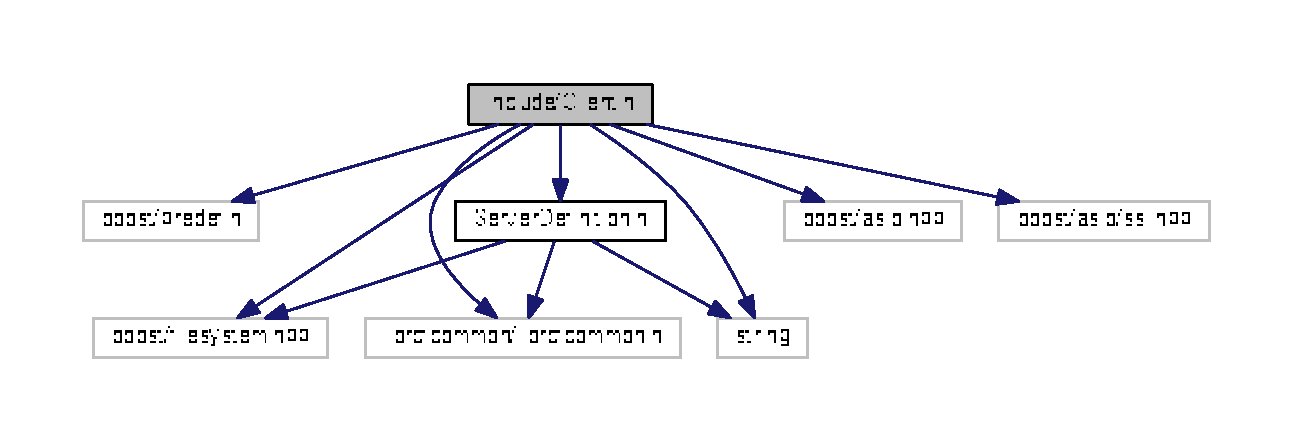
\includegraphics[width=350pt]{_client_8h__incl}
\end{center}
\end{figure}
This graph shows which files directly or indirectly include this file\+:\nopagebreak
\begin{figure}[H]
\begin{center}
\leavevmode
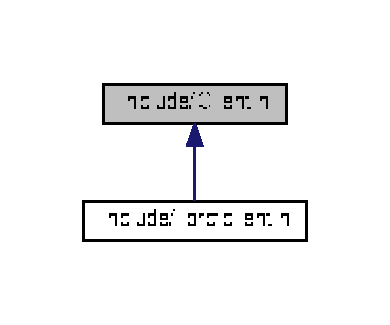
\includegraphics[width=187pt]{_client_8h__dep__incl}
\end{center}
\end{figure}
\subsection*{Classes}
\begin{DoxyCompactItemize}
\item 
class \hyperlink{class_r_c_f_1_1_client_1_1_client}{R\+C\+F\+::\+Client\+::\+Client}
\begin{DoxyCompactList}\small\item\em A class that can be used to create \hyperlink{namespace_r_c_f}{R\+C\+F} client and contains useful \hyperlink{namespace_r_c_f}{R\+C\+F} protocol methods. \end{DoxyCompactList}\end{DoxyCompactItemize}
\subsection*{Namespaces}
\begin{DoxyCompactItemize}
\item 
 \hyperlink{namespace_r_c_f}{R\+C\+F}
\begin{DoxyCompactList}\small\item\em A global namespace for Remote\+Control\+Framework. \end{DoxyCompactList}\item 
 \hyperlink{namespace_r_c_f_1_1_client}{R\+C\+F\+::\+Client}
\begin{DoxyCompactList}\small\item\em A namespace for \hyperlink{namespace_r_c_f}{R\+C\+F} client. \end{DoxyCompactList}\end{DoxyCompactItemize}
\subsection*{Typedefs}
\begin{DoxyCompactItemize}
\item 
\hypertarget{_client_8h_a099e2c9fff985800932f4c424a126989}{}typedef boost\+::asio\+::ssl\+::stream$<$ boost\+::asio\+::ip\+::tcp\+::socket $>$ \hyperlink{_client_8h_a099e2c9fff985800932f4c424a126989}{ssl\+\_\+socket}\label{_client_8h_a099e2c9fff985800932f4c424a126989}

\begin{DoxyCompactList}\small\item\em This is a name simplification for Boost\+::\+Asio\textquotesingle{} s S\+S\+L socket stream type. \end{DoxyCompactList}\end{DoxyCompactItemize}


\subsection{Detailed Description}
A class that can be used to create \hyperlink{namespace_r_c_f}{R\+C\+F} client and contains useful \hyperlink{namespace_r_c_f}{R\+C\+F} protocol methods. 

\begin{DoxyAuthor}{Author}
Phitherek\+\_\+ 
\end{DoxyAuthor}
\begin{DoxyDate}{Date}
2015 
\end{DoxyDate}
\begin{DoxyVersion}{Version}
0.\+1 
\end{DoxyVersion}

\hypertarget{_server_definition_8h}{}\section{include/\+Server\+Definition.h File Reference}
\label{_server_definition_8h}\index{include/\+Server\+Definition.\+h@{include/\+Server\+Definition.\+h}}


A class that represents server definition for client.  


{\ttfamily \#include $<$librcfcommon/librcfcommon.\+h$>$}\\*
{\ttfamily \#include $<$boost/filesystem.\+hpp$>$}\\*
{\ttfamily \#include $<$string$>$}\\*
Include dependency graph for Server\+Definition.\+h\+:\nopagebreak
\begin{figure}[H]
\begin{center}
\leavevmode
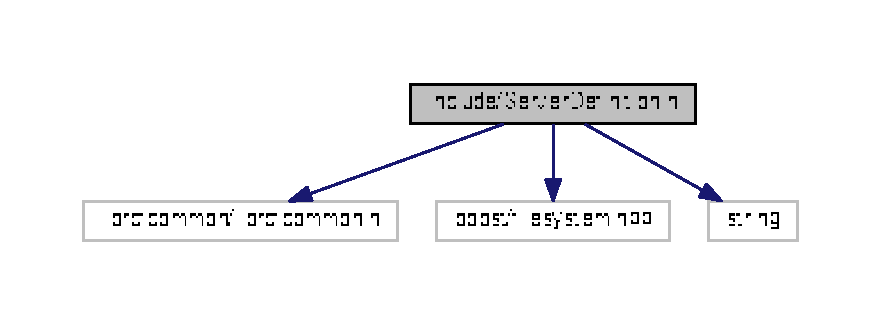
\includegraphics[width=350pt]{_server_definition_8h__incl}
\end{center}
\end{figure}
This graph shows which files directly or indirectly include this file\+:\nopagebreak
\begin{figure}[H]
\begin{center}
\leavevmode
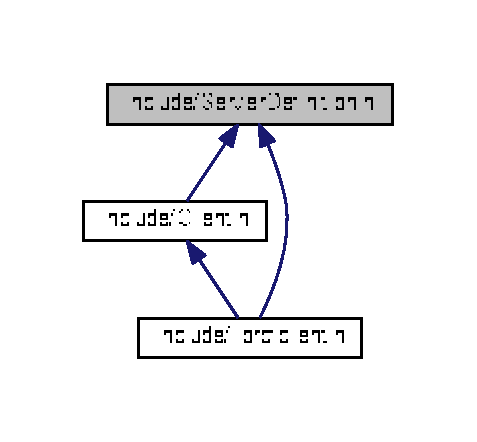
\includegraphics[width=229pt]{_server_definition_8h__dep__incl}
\end{center}
\end{figure}
\subsection*{Classes}
\begin{DoxyCompactItemize}
\item 
class \hyperlink{class_r_c_f_1_1_client_1_1_server_definition}{R\+C\+F\+::\+Client\+::\+Server\+Definition}
\begin{DoxyCompactList}\small\item\em A class that represents server definition for client. \end{DoxyCompactList}\end{DoxyCompactItemize}
\subsection*{Namespaces}
\begin{DoxyCompactItemize}
\item 
 \hyperlink{namespace_r_c_f}{R\+C\+F}
\begin{DoxyCompactList}\small\item\em A global namespace for Remote\+Control\+Framework. \end{DoxyCompactList}\item 
 \hyperlink{namespace_r_c_f_1_1_client}{R\+C\+F\+::\+Client}
\begin{DoxyCompactList}\small\item\em A namespace for \hyperlink{namespace_r_c_f}{R\+C\+F} client. \end{DoxyCompactList}\end{DoxyCompactItemize}


\subsection{Detailed Description}
A class that represents server definition for client. 

\begin{DoxyAuthor}{Author}
Phitherek\+\_\+ 
\end{DoxyAuthor}
\begin{DoxyDate}{Date}
2015 
\end{DoxyDate}
\begin{DoxyVersion}{Version}
0.\+1 
\end{DoxyVersion}

%--- End generated contents ---

% Index
\backmatter
\newpage
\phantomsection
\clearemptydoublepage
\addcontentsline{toc}{chapter}{Index}
\printindex

\end{document}
